\chapter{Wstęp}

\section{Transport okazjonalny}
Transport towarów odgrywa kluczową rolę w globalnej gospodarce, łącząc producentów, dystrybutorów i konsumentów na całym świecie. Efektywność transportu ma bezpośredni wpływ na koszty operacyjne firm oraz na ceny finalnych produktów. W zależności od specyfiki przewożonych towarów oraz potrzeb zleceniodawców, transport może przyjmować dwie formy:

\label{sec:przewoz_regularny}
Transport regularny to przewóz towarów, który odbywa się według ustalonego harmonogramu i stałych tras. Charakteryzuje się regularnością kursów, co oznacza, że pojazdy wykonują swoje trasy w określonych, z góry ustalonych terminach. Przykładami transportu regularnego są linie autobusowe, kolejowe czy lotnicze, które działają według stałego rozkładu jazdy.

\label{sec:transport_okazjonalny}
Transport okazjonalny to przewóz towarów, który nie spełnia definicji przewozu regularnego. Oznacza to, że odbywa się on bez ustalonego z góry rozkładu jazdy i może dotyczyć zarówno tras krajowych, jak i międzynarodowych. Pojazdy wykonują swoje trasy w zależności od zapotrzebowania klientów. Sam przewóz zaś zlecany jest na potrzebę klienta, nie musi on jednak określnać dokładnego terminu odbycia trasy, ani przez kogo ma on być zrealizowany.

Podczas swoich tras przewoźnicy czasami są zmuszeni do powrotu z miejsca docelowego bez żadnego załadunku. Powoduje to, że trasy nie są w pełni zoptymalizowane względem kosztów, jakie niesie za sobą pokonywana trasa. Możliwe jest jednak zredukowanie występowania takich sytuacji poprzez odpowiednie powiązanie przewoźników i osób zlecających transport. Zleceniodawca, który nie potrzebuje dostawy towaru w konkretnej dacie, mógłby wtedy zlecić transport z nieokreślonym dokładnie terminem dotarcia towaru, w zamian za niższe ceny przewozowe. Przykład: dyrektor szkoły, w czasie wakacji, zamówił dużych rozmiarów tablicę interaktywną, która nie zmieściłaby się w standardowym samochodzie osobowym. Z racji, że zamówienie zostało złożone w czasie, gdy dzieci nie chodzą do szkoły, nie zależy mu na dokładnej dacie dostawy. Może on w takim przypadku zlecić dostawę tablicy w formie transportu okazjonalnego, z mniejszymi kosztami transportu. Przewoźnik przeglądający takie zlecenia mógłby zabrać towar i zawieźć go na miejsce docelowe, gdy akurat odbywałby trasę bez załadunku i kierował się w tym przybliżonym kierunku.

Połączenie między zleceniodawcami, a przewoźnikami, może odbywać się za pomocą serwisu oferującego dodawanie publicznych ogłoszeń przez obie strony. Prowadziłoby to do sytuacji, w której obie strony korzystają. Przewoźnicy, ponieważ zmniejszyło by to występowanie tras bez załadunku, tym samym zwiększając zyski z tras powrotnych. Zleceniodawcy, natomiast generują mniejsze koszty, związane z brakiem konieczności korzystania z droższych określonych terminowo usług transpotowych.

\label{sec:cele}
\section{Cel projektu}
Celem projektu jest stworzenie aplikacji webowej pozwalającej na dodawanie ogłoszeń transportów okazjonalnych, która zoptymalizuje procesy logistyczne i wyeliminuje nieefektywne wykorzystanie zasobów transportowych. Aplikacja umożliwi użytkownikom łatwe i szybkie znalezienie odpowiedniego przewoźnika lub zleceniodawcy, co spowoduje redukcje pustych przebiegów i tym samym kosztów transportu.
Główne cele projektu:
\begin{enumerate}
    \item \textbf{Ułatwienie szukania odpowiednich ofert}, poprzez system dopasowywania zleceń transportowych do planownych tras przewoźników, aplikacja usprawni komunikację między zleceniodawcami a przewoźnikami, skracając czas potrzebny na znalezienie odpowiedniego transportu.
    \item \textbf{Eliminacja pustych przebiegów}, aplikacja umożliwi przewoźnikom znalezienie ładunków na trasach powrotnych, co zmniejszy liczbę pustych przebiegów, przyczyniając się tym do wyższej efektywności wykorzystania zasobów.
    \item \textbf{Redukcja kosztów transportu}, dzięki lepszemu dopasowaniu potencjalnych kontrahentów dla usług transportowych, aplikacja pozwoli na obniżenie kosztów transportu zarówno dla zleceniodawców, jak i przewoźników.
\end{enumerate}
Nowoczesna aplikacja transportowa przyczyni się do efektywnego zrealizowania tych celów, co wspomoże rynek zleceń transportowych, przynosząc korzyści zarówno dla zleceniodawców, jak i przewoźników.

\section{Wymagania aplikacji}
Analizując cele wymienione w podrozdziale \hyperref[sec:cele]{1.1} oraz opis samej aplikacji, można wywnioskować, że do efektywnego działania serwisu, będą musiały zostać zrealizowane następujące wymagania funkcjonalne:
\begin{enumerate}
    \item Dodawanie ogłoszeń o planowanej trasie: system powinien pozwalać przewoźnikom, na dodawanie publicznych informacji o planowanych przez siebie trasach. Ogłoszenie będzie składało się z:
    \begin{itemize}
        \item planowanej trasy (punkty A i B na mapie),
        \item daty planowanej trasy,
        \item dostępnego miejsca w pojeździe (wymiary liczone w europaletach),
        \item maksymalnej wagi towaru,
        \item danych kontaktowych,
        \item imienia i nazwiska przewoźnika,
        \item oceny przewoźnika, wraz z komentarzami,
        \item opisu ogłoszenia (niewymagane),
    \end{itemize}
    \item Dodawanie zleceń transportowych: zleceniodawcy powinni mieć możliwość zlecenia przewozu towaru, serwis pomagał będzie znaleźć odpowiedniego przewoźnika, poprzez udostępnienie możliwości dodania ogłoszenia zlecenia. W ogłoszeniu zlecenia znajdować się będzie:
    \begin{itemize}
        \item wymagana trasa (punkty A i B na mapie),
        \item termin dostarczenia (przedział dat),
        \item waga towarów do przewiezenia,
        \item wymiary przewożonych dóbr,
        \item kategoria każdego z towarów,
        \item informacja o specjalnych warunków podczas transportu (niewymagane),
        \item wynagrodzenie (z zaznaczeniem czy kwota podlega negocjacji),
        \item pseudonim autora,
        \item ocena zleceniodawcy, wraz z komentarzami,
        \item opis zlecenia (niewymagane),
    \end{itemize}
    \item Uwierzytelnianie: aplikacja będzie wykorzystywała system rejestracji oraz logowania.
    \item System rekomendacji ofert: podczas wprowadzania danych o trasie, użytkownik będzie informowany o sugerowanych zleceniach dodanych przez innych użytkowników (np. gdy zlecenie dotyczy trasy, która przewoźnik planuje się poruszać).
    \item Umożliwienie konaktu między użytkownikami: jednym z założeń projektowych jest dodanie czatu tekstowego umożliwiającego korespondencje między zleceniodawcami, a przewoźnikami, bezpośrednio w aplikacji. Ma on pełnić rolę komunikacji na wzór tej  oferowanej przez tradycyjną poczte elektroniczną.
    \item Podpisywanie umowy: użytkownicy, po negocjacji warunków umowy, otrzymają wygenerowany przez serwis dokument finalizujący transakcje.
    \item Weryfikacja dodawanych ogłoszeń: zanim ogłoszenie wyświetlać się będzie dla wszystkich użytkowników, wymagana będzie akceptacja jednego z moderatorów serwisu.
    \item Graficzne przedstawienie trasy: w ogłoszeniach dodanych przez użytkowników, wyświetlana będzie mapa z zaznaczoną trasą. Ułatwi to użytkownikom zobrazowanie planowanego kursu.
\end{enumerate}
Aplikacja powinna być niezawodna i przyjazna do użytkowania dla wszystkich. Do komfortowego korzystania z serwisu przez użytkowników, niezbędna będzie realizacja następujących wymagań niefunkcjonalnych
\begin{enumerate}
    \item Innowacyjność: wykorzystanie nowoczesnych technologii, takich jak \texttt{TypeScript}, \texttt{Next.js}, \texttt{Tailwind CSS}, \texttt{Node.js} oraz \texttt{PostgreSQL}, zapewni wysoką wydajność, skalowalność i bezpieczeństwo aplikacji.
    \item Intuicyjny interfejs użytkownika: Aplikacja będzie posiadać prosty i intuicyjny interfejs użytkownika, który umożliwi łatwą obsługę zarówno dla zleceniodawców, jak i przewoźników.
    \item Dostępność na różnych urządzeniach: Aplikacja będzie responsywna i dostosowana do różnych urządzeń, takich jak komputery, tablety i smartfony, co zapewni wygodę użytkowania w dowolnym miejscu i czasie.
    \item Wielojęzyczność: użytkownicy korzystający z aplikacji, będą mieli możliwość wyboru jednego z trzech przewidzianych języków: polski, angielski oraz niemiecki. Co przełoży się na międzynarodowy aspekt aplikacji.
    \item Regulanim: podczas rejestrowania się do serwisu, użytkownik musi zaakceptować regulamin korzystania z aplikacji. Zabezpieczy to aplikacje od strony prawnej.
\end{enumerate}

\section{Przypadki użycia}
Biorąc pod uwagę założenia opisane w poprzednich podrozdziałach, zaprojektowany został diagram przypadków użycia aplikacji. Idnetyfikacja aktorów:
\begin{enumerate}
\item Użytkownik - ogólny użytkownik systemu. Reprezentuje dowolną osobę korzystającą z serwisu, jego przypadki użycia będą dziedziczone przez pozostałych aktorów systemu.
\begin{figure}[H]
	\centering
		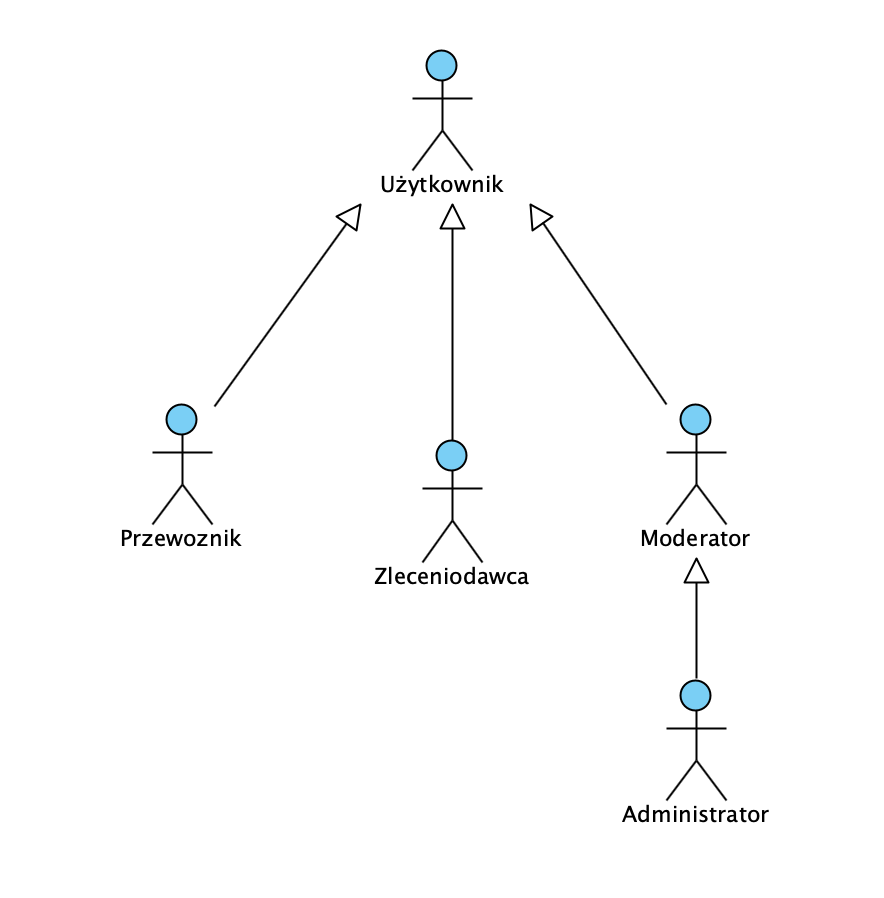
\includegraphics[width=0.6\linewidth]{rozdzial1/dziedziczenie.png}
	\caption{Graficzne ukazanie dziedziczenia możliwości aktorów}
	\label{Rys. fig:Graficzne ukazanie dziedziczenia możliwości aktorów}
\end{figure}
\item Przewoźnik - aktor odpowiedzialny za transport towarów. Może przeglądać dostępne zlecenia, dodawać ogłoszenia o planowanych trasach, komunikować się z autorami ogłoszeń, przyjmować zlecenia oraz oceniać i komentować kontrahentów.
\item Zleceniodawca - użytkownik systemu, który zleca transport towarów. Może dodawać nowe zlecenia transportowe, podobnie jak przewoźnik, może również przeglądać ogłoszenia przewoźników oraz komunikować się z autorami ogłoszeń.
\item Moderator - osoba odpowiedzialna za zarządzanie systemem. Moderator zatwierdza lub usuwa nowe ogłoszenia i zlecenia oraz blokuje konta użytkowników.
\item Administrator - użytkownik umiejscowiony najwyżej w hierarchii systemu. Może on wykonywać wszystko co moderator, lecz ma również możliwość dodawania nowych moderatorów lub usuwania obecnych.
\end{enumerate}

\begin{figure}[H]
	\centering
		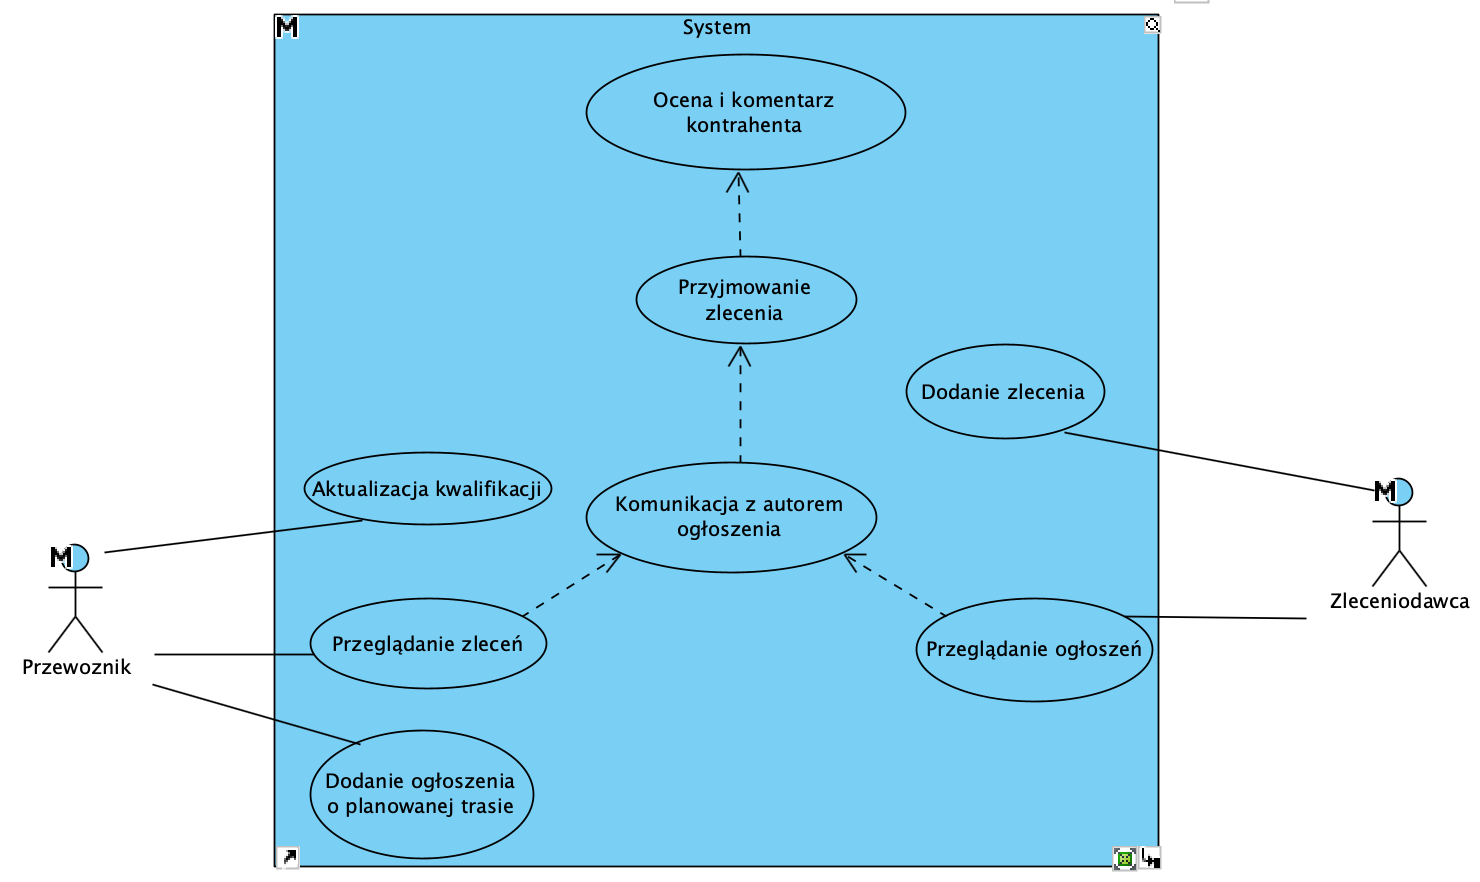
\includegraphics[width=0.9\linewidth]{rozdzial1/glowne_zalozenia.png}
	\caption{Diagram głównych funkcjonalności aplikacji}
	\label{Rys. fig:Diagram głównych funkcjonalności aplikacji}
\end{figure}

Na powyższym obrazku przedstawiony został diagram przypadków użycia dla przewoźnika oraz zleceniodawcy.

\begin{figure}[H]
	\centering
		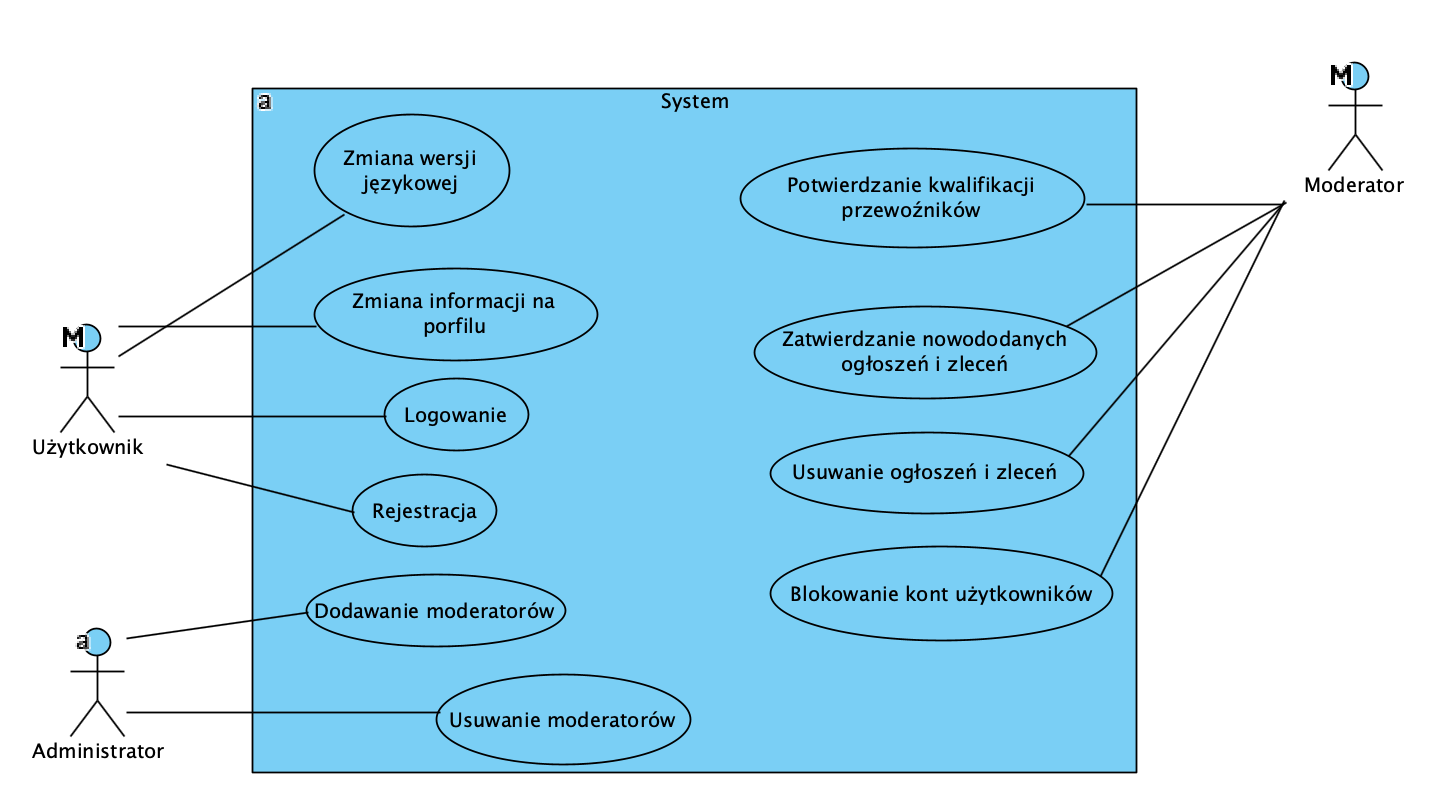
\includegraphics[width=0.9\linewidth]{rozdzial1/ogolny_schemat.png}
	\caption{Główne założenia projektowe od strony zarządzania serwisem}
	\label{Rys. fig:Główne założenia projektowe od strony zarządzania serwisem}
\end{figure}

Diagram ukazujący główne założenia systemu od strony zarządzania serwisem, w tym możliwości użytkownika, moderatora oraz administratora.
